\documentclass[10pt]{article}
\usepackage{xspace}
\usepackage{graphicx}
\setlength{\topmargin}{-0.5in}
\setlength{\oddsidemargin}{0.0in}
\setlength{\evensidemargin}{0.0in}
\setlength{\textheight}{9in}
\setlength{\textwidth}{6.5in}

\renewcommand{\thepage}{p. \arabic{page} \quad -- \quad 03/25/2005}

\newcommand{\bing}{{\bf BING!} }
\newcommand{\goto}[1]{\bing \vskip 12pt \section*{{\em{#1}}}}
\newcommand{\ps}{ plus Spehn\xspace}
\begin{document}

\begin{center}

MIT Science Fiction Society 

84 Massachusetts Avenue

Cambridge, MA 02139

\vspace{12pt}

MITSFS Meeting Minutes 

Friday, March 25, 2005

\end{center}
 
\vspace{18pt}

\setlength{\parskip}{6pt}

\noindent
MITSFS meeting called to order, 1730 SST, Andrew Clough, Pseudo-Skinner, presiding; Ash Turza,  Pseudo-Onseck, recording.

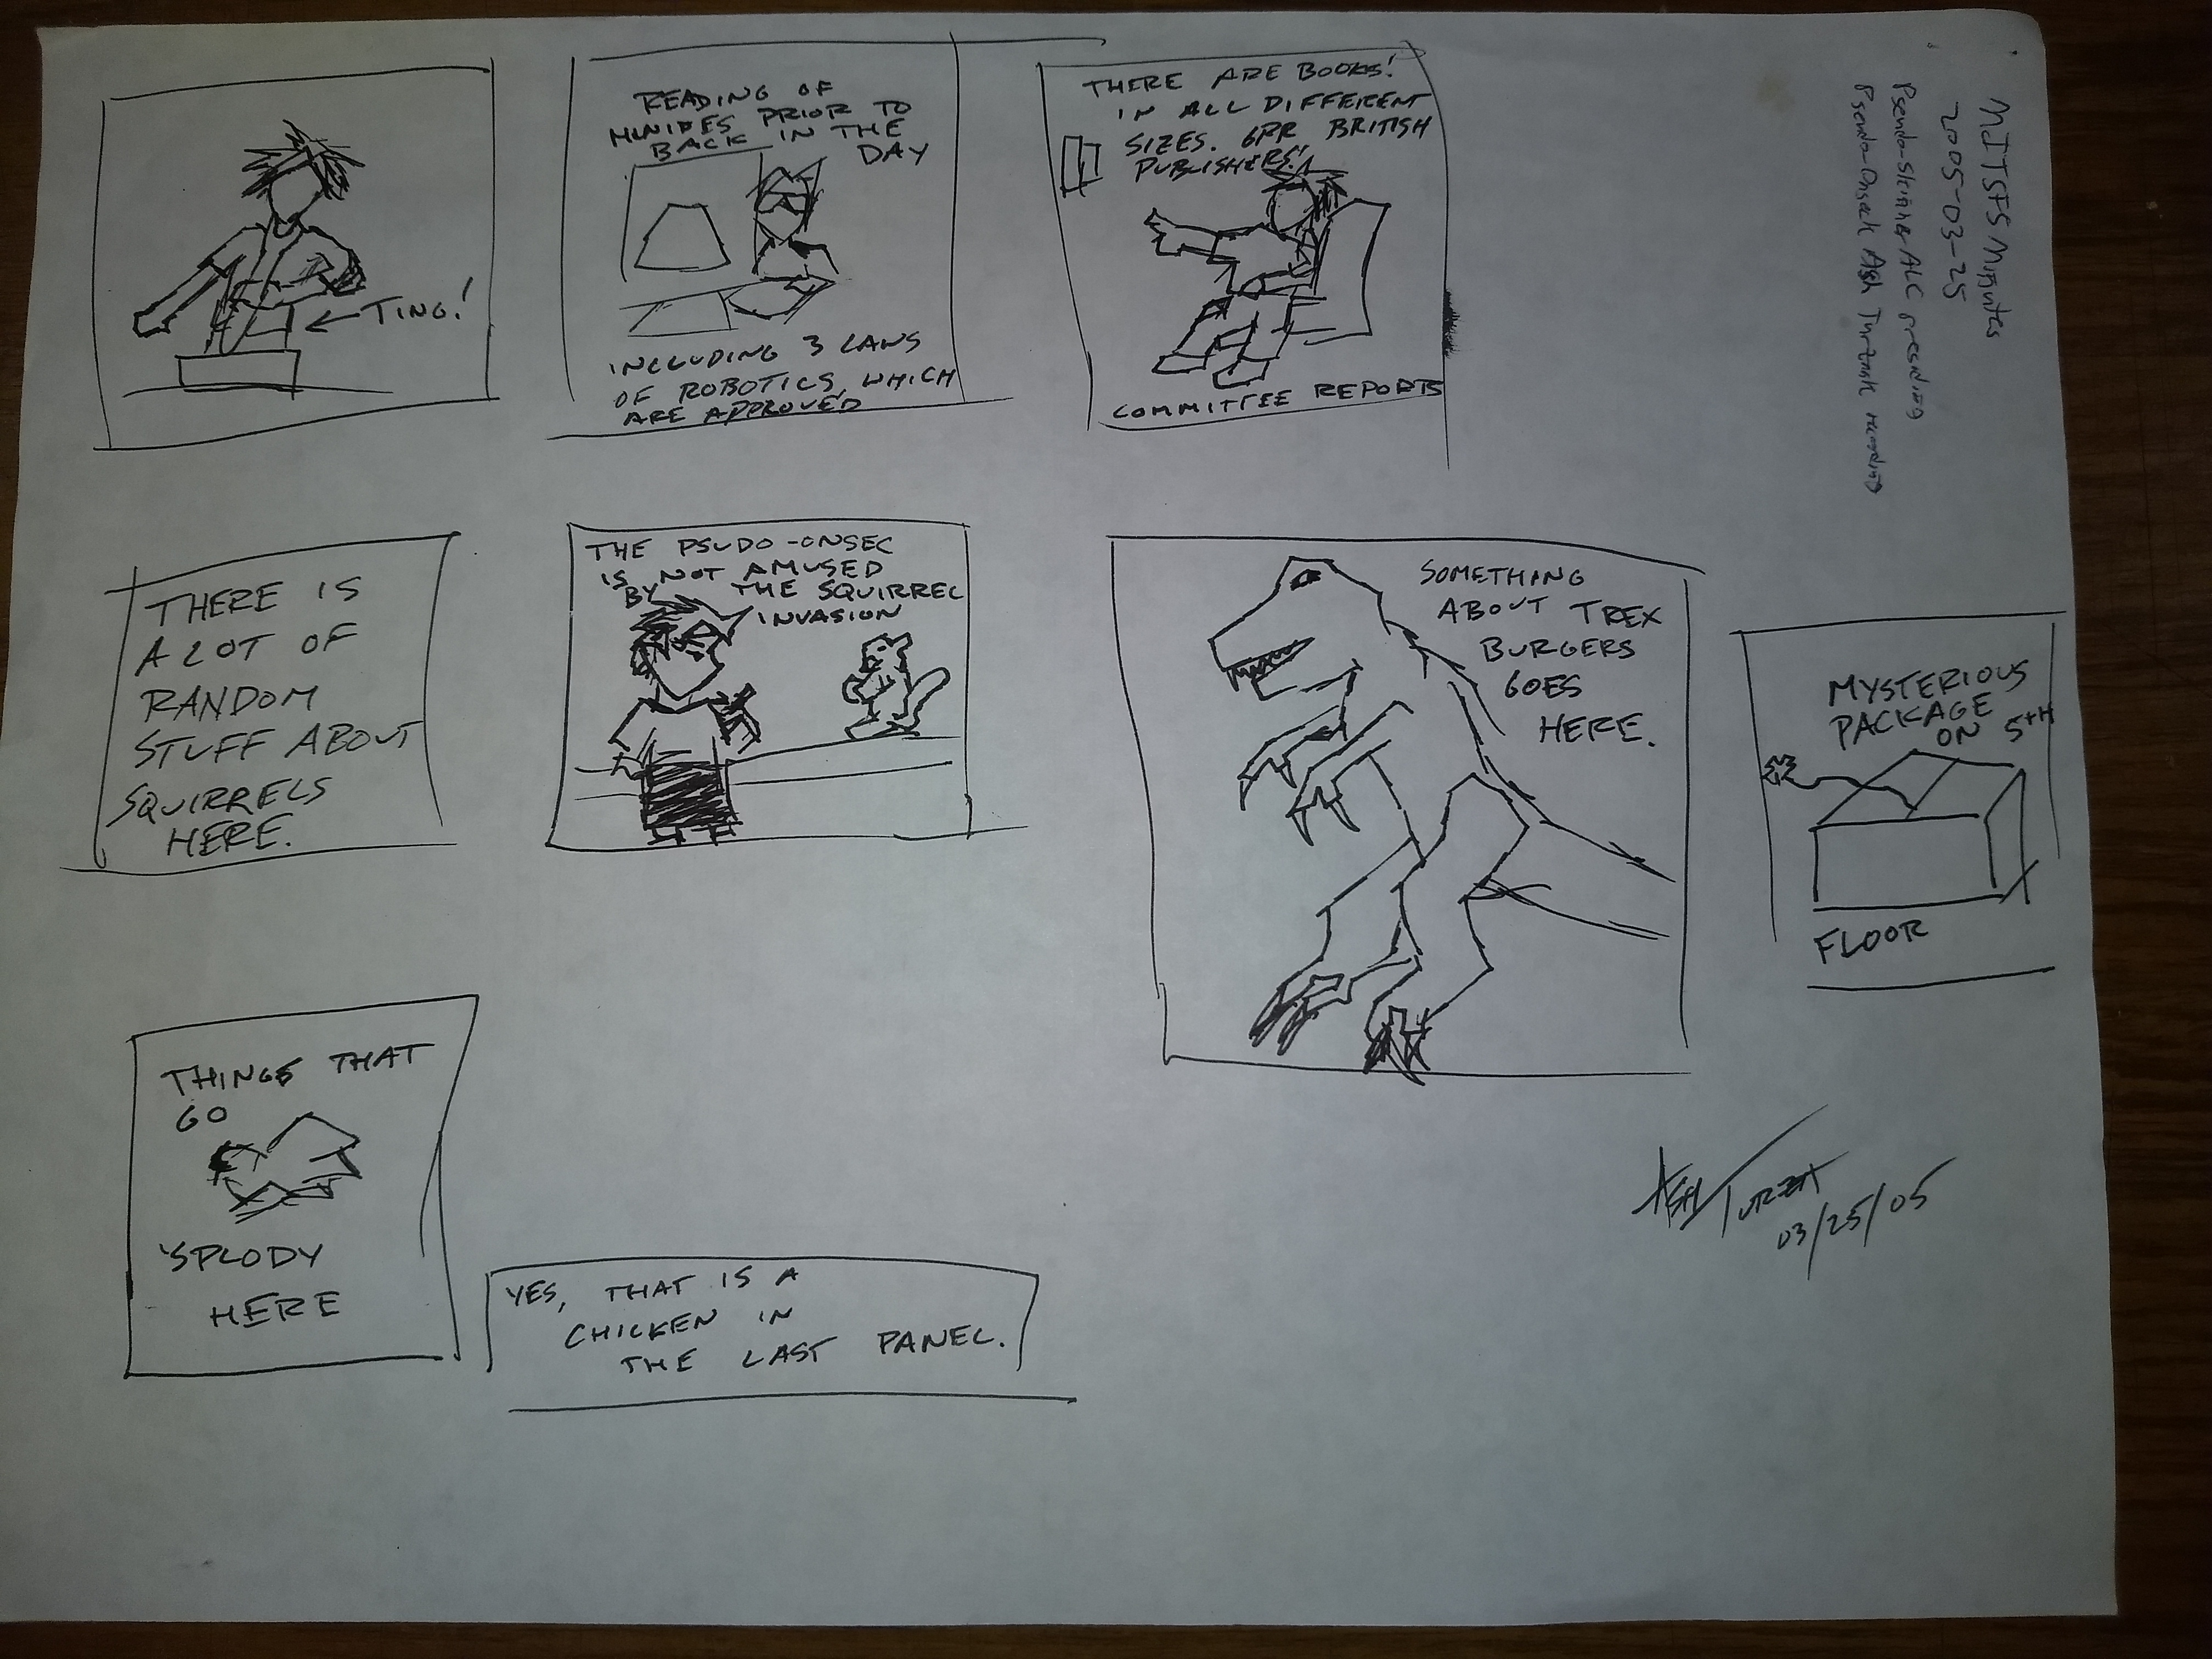
\includegraphics[scale=0.3]{/afs/athena.mit.edu/activity/m/mitsfs/minutes/2005/panel-2005-03-25-01.jpg} 

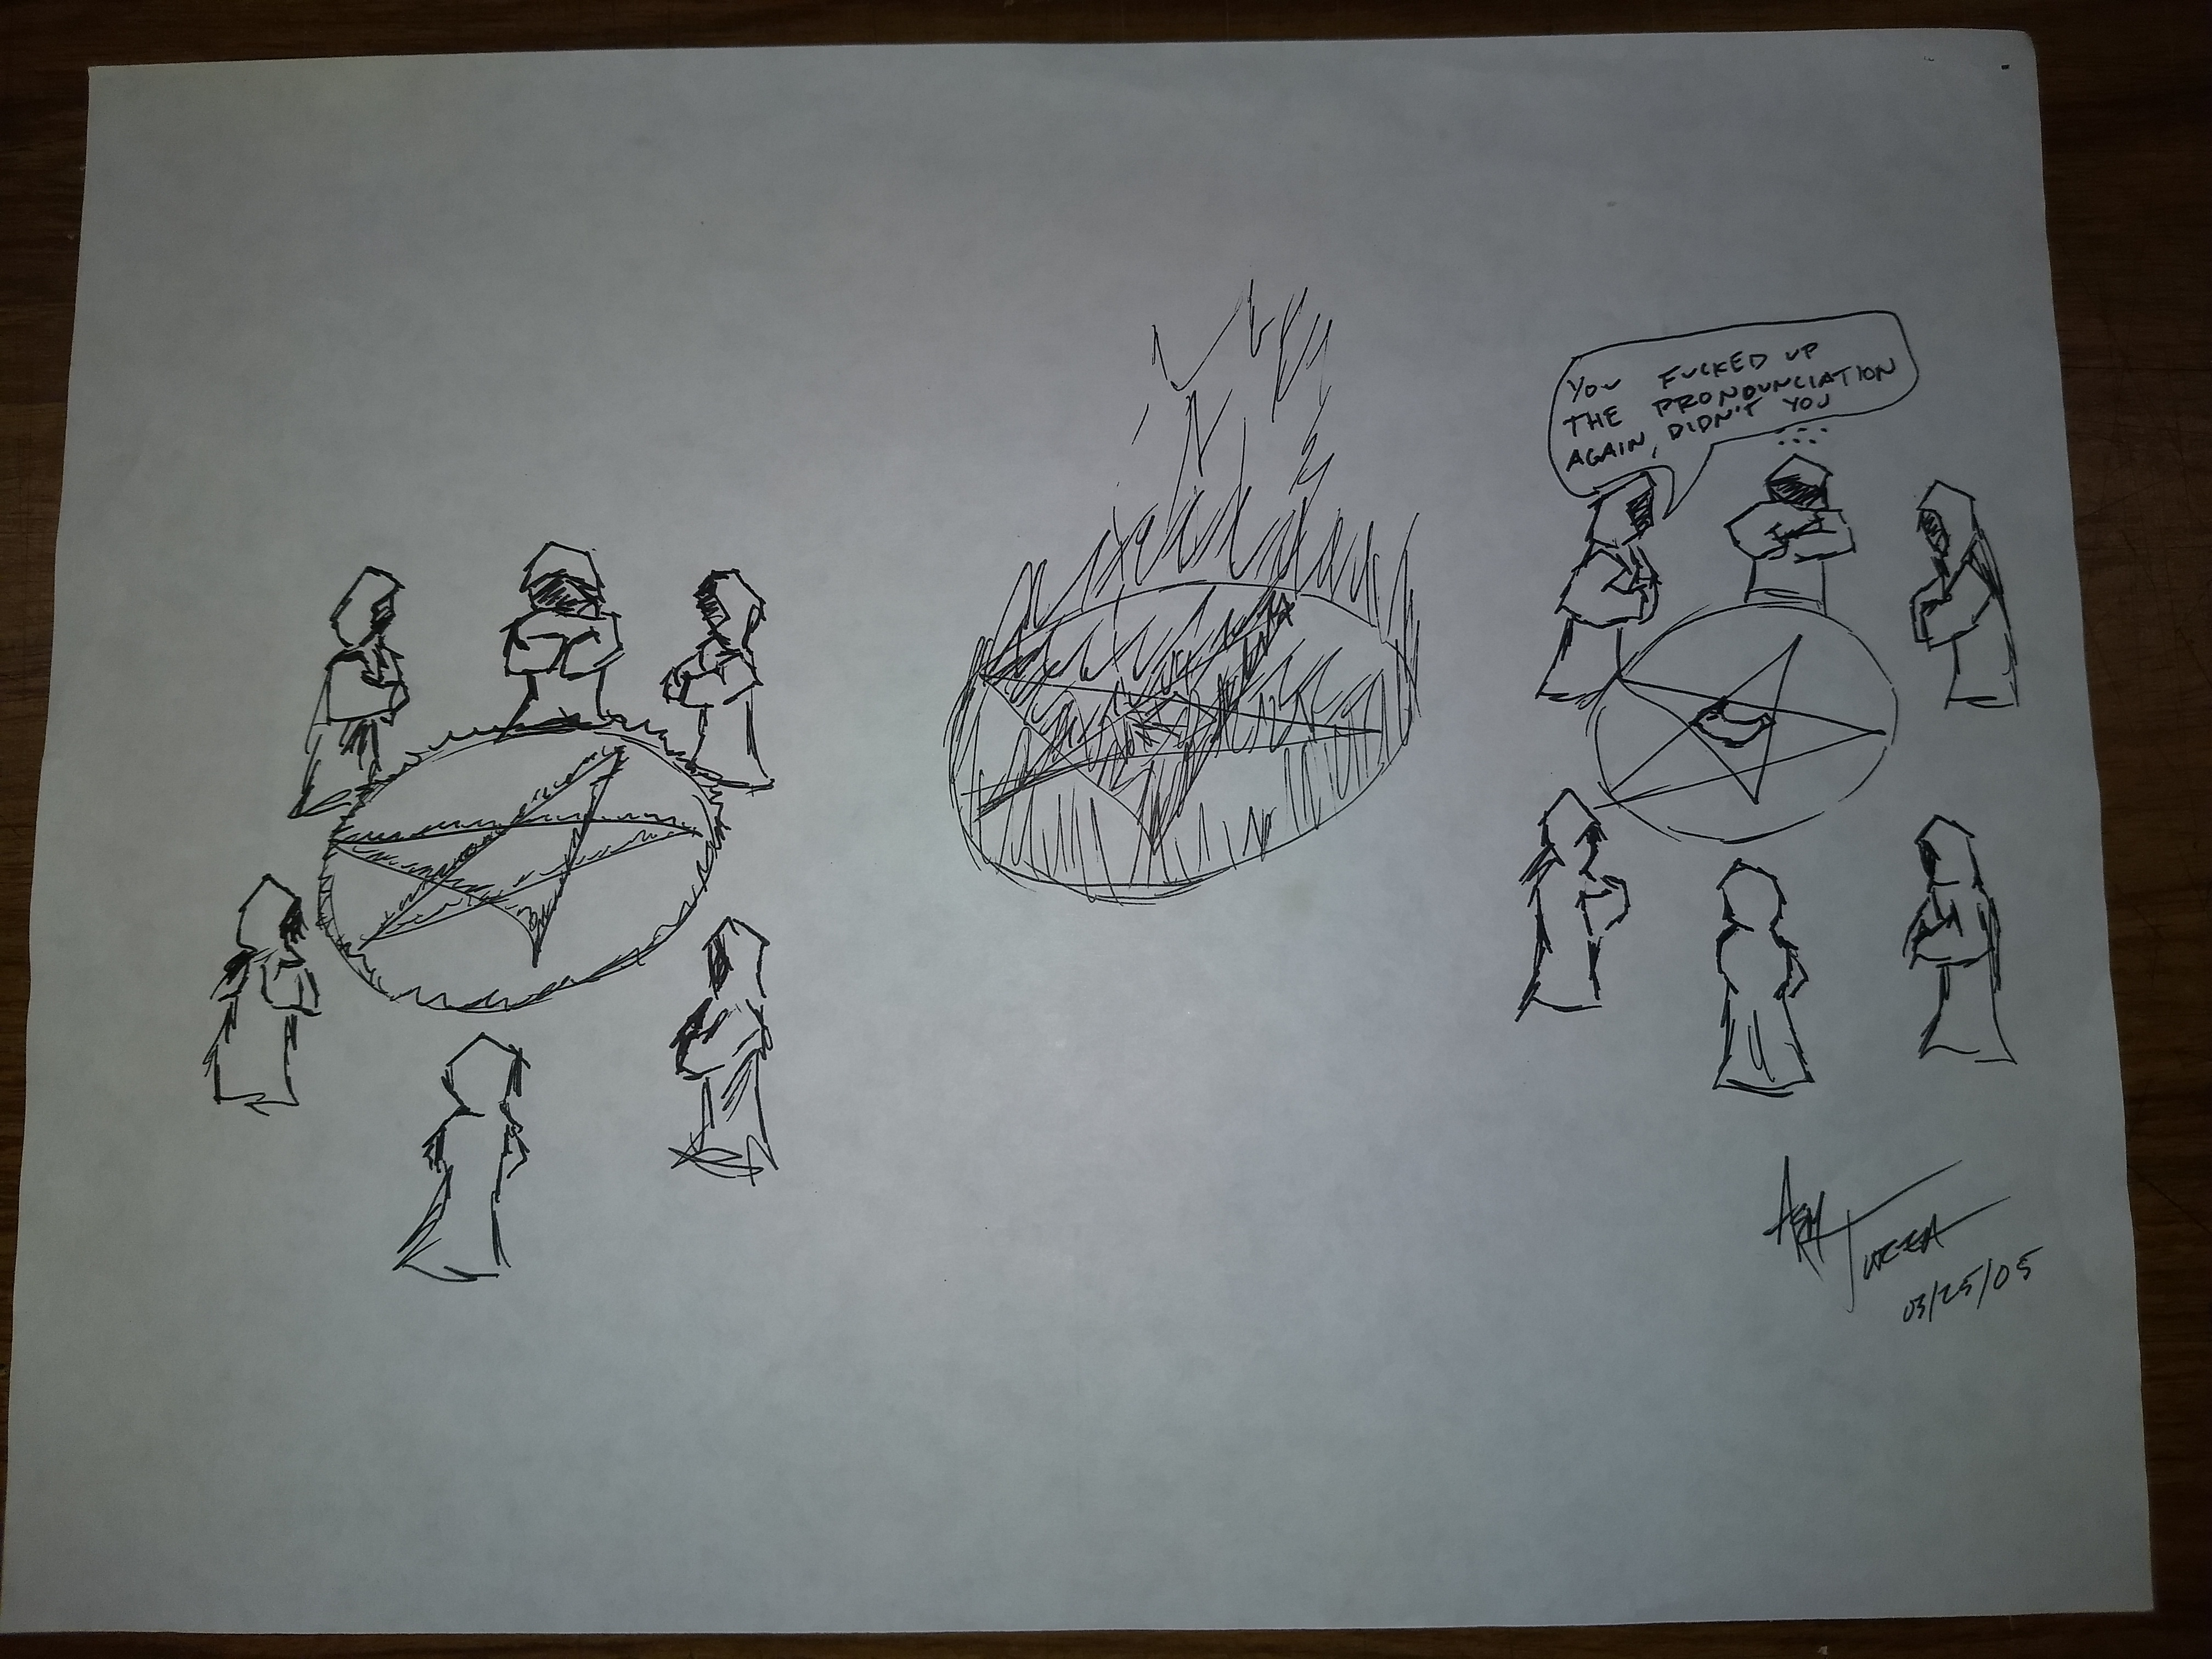
\includegraphics[scale=0.3]{/afs/athena.mit.edu/activity/m/mitsfs/minutes/2005/panel-2005-03-25-02.jpg} 

\vspace{12pt}

\noindent
Meeting adjourned, 1800 SST.

\vspace{18pt}

\centerline{Respectfully submitted,}
\centerline{Ash Turza, Pseudo-Onseck}

\end{document}
